\documentclass[letterpaper, 12pt]{book}
\usepackage[margin=1in]{geometry}
\usepackage[acronym]{glossaries}
\usepackage{xcolor}
\usepackage{amsmath}
\usepackage{multicol}
\usepackage{enumitem}
\usepackage{tikz}
\usepackage{arabxetex}
\usepackage{xeCJK}
\usepackage{CJKnumb}

\usetikzlibrary{shapes.geometric, arrows}
\tikzstyle{rec} = [rectangle,minimum width=3cm, minimum height=1cm,text centered, draw=black]
\tikzstyle{arrow} = [thick,->,>=stealth]
\tikzstyle{darrow} = [thick,<->,>=stealth]

\makeglossaries


\newacronym{msb}{MSB}{most significant bit}
\newacronym{lsb}{LSB}{least significant bit}
\newacronym{ip}{IP}{instruction pointer}
\newacronym{risc}{RISC}{reduced instruction set computer}
\newacronym{cisc}{CISC}{complex instruction set computer}
\newglossaryentry{overflow}{name=overflow,description={%
    Exceeding the capacity of a binary number with fixed number of digits
}}
\newglossaryentry{unsigned}{name=unsigned,description={%
    A data type that allows for only positive numbers or operation that assumes the operands are positive numbers
}}
\newglossaryentry{von Neumann architecture}{name=von Neumann architecture,description={%
    An electronic digital computer possessing an arithmetic logic unit, a control unit, memory, input and output
}}
\newglossaryentry{arithmetic logic unit}{name={arithmetic logic unit},%
    description={The component of a microprocessor responsible for computing arithmetic},%
    first={\glsentryname{arithmetic logic unit} (ALU)}
}
\newglossaryentry{register}{name={register},%
    description={Fast temporary storage physically located on the microprocessor}
}
\newglossaryentry{control unit}{name={control unit},%
    description={The component of a microprocessor that controls the operation of the microprocessor}
}
\newglossaryentry{instruction register}{name={instruction register},%
    description={A register in the microprocessor that holds the value of the current instruction}
}
\newglossaryentry{instruction pointer}{name={instruction pointer},%
    description={A register in the microprocessor that holds the address of the next instruction to be executed},%
    first={\glsentryname{instruction pointer} (IP)}
}
\newglossaryentry{Harvard architecture}{name={Harvard architecture},%
    description={A model for computing that differs from the von Neumann architecture by distinguishing between instruction memory and data memory}
}
\newglossaryentry{cache}{name={cache},%
    description={An intermediate memory structure between the memory and the microprocessor designed to improve the speed of memory operations}
}
\newglossaryentry{reduced instruction set computer}{name={RISC},%
    description={A simple microprocessor where instructions generally perform only singular actions resulting in a smaller instruction set},%
    first={reduced instruction set computer (RISC)}
}
\newglossaryentry{complex instruction set computer}{name={CISC},%
    description={A complicated type of microprocessor with a large instruction set where a single instruction may be capable of performing multiple operations at once},%
    first={complex instruction set computer (CISC)}
}
\newglossaryentry{load-and-store}{name={load-and-store architecture},%
    description={A type of architecture where memory operations are distinct from other types of operations}
}
\newglossaryentry{register-memory}{name={register-memory architecture},%
    description={A type of architecture where operations can reference memory without need of additional memory operations}
}
\newglossaryentry{aarch64}{name={ARM64},%
    description={The 64-bit extension of the Advanced/Acorn RISC machine (ARM) architecture family, also known as ARM64},%
    first={Acorn RISC Machine (ARM64)}
}
\newglossaryentry{x64}{name={AMD64},%
    description={The 64-bit extension of the x86-architecture, backward compatible with x86, also known as x86-64}
}
\newglossaryentry{x86}{name={x86},%
    description={The 32-bit version of the x86-architecture, sometimes written as x86-32}
}
\newglossaryentry{isa}{name={ISA},%
    description={Instruction set architecture. The term for a specific microprocessor design, and its set of instructions},%
    first={instruction set architecture (ISA)}
}
\newglossaryentry{edvac}{name={EDVAC},%
    description={Electronic Discrete Variable Automatic Computer, one of the earliest electronic computers},%
    first={Electronic Discrete Variable Automatic Computer (EDVAC)}
}
\newglossaryentry{control of flow}{name={control of flow},%
    description={A type of operation that causes the microprocessor to execute some other instruction, other than the next one}
}
\newglossaryentry{ia64}{name={IA-64},%
    description={An instruction set architecture originally developed by HP and proposed as a 64-bit alternative to x86 by Intel},%
    first={Itanium (IA-64)}%
}
\newglossaryentry{calling convention}{name={calling convention},%
    description={A set of requirements based on the operating system and ISA defining standards for how to use the registers and stack}
}
\newglossaryentry{temporal locality}{name={temporal locality},%
    description={The concept that if a value from memory is accessed it has a high probability of being accessed again}
}
\newglossaryentry{dram}{name={DRAM},%
    description={Dynamic random access memory, a simple type of memory technology that has difficulties with random access},%
    first={dynamic random access memory (DRAM)}%
}
\newglossaryentry{sram}{name={SRAM},%
    description={Static random access memory, a fast but comparatively expenstive type of memory technology}
}
\newglossaryentry{sp}{name={SP},%
    description={Stack pointer, pointing the the next available space on the stack},%
    first={stack pointer (SP)}
}
\newglossaryentry{fp}{name={FP},%
    description={Frame pointer, pointing the the procedure call's current frame},%
    first={frame pointer (FP)}
}
\newglossaryentry{reference zero}{name={reference zero},
    description={A special register that will be read as zero when used as an operand, or will throw away the result if used as a destination}
}
\newglossaryentry{ra}{name={RA},%
    description={The return address, points to where a procedure call should return on completion},%
    first={return address (RA)}
}
\newglossaryentry{callee}{name={callee},%
    description={When a subroutine calls another subroutine, the callee is the subroutine that has been called}
}
\newglossaryentry{caller}{name={caller},%
    description={When a subroutine calls another subroutine, the caller is the subroutine initating the call}
}
\newglossaryentry{powerpc}{name={PowerPC},%
    description={A microprocessor made by IBM briefly used as the microprocessor for Macintosh computers}
}
\newglossaryentry{intel}{name={Intel},%
    description={A semiconductor manufacturer, developed the x86 ISA}
}   
\newglossaryentry{amd}{name={AMD},%
    description={Advanced Micro Devices, a semiconductor manufacturer, developed the AMD64 ISA}
}
\newglossaryentry{stored program computer}{name={stored program computer},%
    description={A system that executes programs in memory, in contrast to computers designed to execute fixed programs}
}
\newglossaryentry{floating point unit}{name={FPU},%
    description={A special purpose ALU that operates on floating-point values},%
    first={floating point unit (FPU)}
}
\newglossaryentry{gpu}{name={GPU},%
    description={A special purpose ALU optimized for executing math operations commonly used in computer graphics applications},%
    first={graphics processing unit (GPU)}
}
\newglossaryentry{opcode}{name={opcode},%
    description={Input to the ALU description the type of operation to be carried out},%
    first={operation code, also known as opcode,}
}
\newglossaryentry{sign and magnitude}{name={sign and magnitude},%
    description={A format for storing positive and negative binary numbers that uses a bit to indicate if the number is positive or negative}
}
\newglossaryentry{floating point number}{name={floating point number},%
    description={A method for storing fractional numbers in binary similar to scientific notation}
}
\newglossaryentry{magnitude}{name={magnitude},%
    description={The absolute value of a number}
}
\newglossaryentry{base-10}{name={base-10},%
    description={Base-10 numbering system also known as decimal, Hindu-Arabic or Western Arabic}
}
\newglossaryentry{base-2}{name={base-2},%
    description={Base-2 numbering system also known as binary}
}

\newcommand*{\example}[1]{\noindent
    \colorbox{blue!10}{\noindent
        \begin{minipage}{\textwidth}
            \textbf{Example \thechapter.\arabic{examples}}\stepcounter{examples}
            #1
        \end{minipage}
    }
}

\newcommand*{\lemma}[1]{\noindent
    \colorbox{green!10}{\noindent
        \begin{minipage}{\textwidth}
            \textbf{Lemma \thechapter.\arabic{examples}}\stepcounter{lemma}
            #1
        \end{minipage}
    }
}

\newcommand*{\myaside}[2]{\noindent
    \colorbox{red!10}{\noindent
        \begin{minipage}{\textwidth}
            \textbf{Aside: #1} 
            #2
        \end{minipage}
    }
}

\begin{document}


\newcounter{examples}{1}
\newcounter{lemma}{1}

\section{Preface\label{sec:preface}}

This textbook is an open-source document that meets the requirements of COMP 142 Computer Architecture and Organization. The goal of the class is to study the organization and behavior of real computer systems at the assembly-language level, the mapping of statements and constructs in a high-level language onto sequences of machine instructions is studied, as well as the internal representation of simple data types and structures. It also covers numerical computation, noting the various data representation errors and potential procedural errors.

The general topics covered by the class are:

\begin{enumerate}
\item Bits, bytes, and words
\item Numeric data representation and number bases
\item Fixed- and floating-point systems
\item Signed and twos-complement representations
\item Representation of nonnumeric data (character codes, graphical data)
\item Representation of records and arrays
\item Basic organization of the von Neumann machine
\item Control unit; instruction fetch, decode, and execution
    Instruction sets and types (data manipulation, control, I/O)
\item Assembly/machine language programming
\item Instruction formats
\item Addressing modes
\item Subroutine call and return mechanisms
\item I/O and interrupts
\end{enumerate}



\chapter{Number Bases\label{sec:numbers}}
\setcounter{examples}{1}

A positional system is a numeral system in which the contribution of a digit to the value of a number 
is the value of the digit multiplied by a factor determined by the position of the digit. In early 
numeral systems, such as Roman numerals, a digit has only one value: I means one, X means ten and C 
a hundred (however, the value may be negated if placed before another digit). In modern positional 
systems, such as the decimal system, the position of the digit means that its value must be multiplied 
by some value: in 555, the three identical symbols represent five hundreds, five tens, and five units, 
respectively, due to their different positions in the digit string. 

Among the earliest systems was the Babylonian numeral system. It used base 60. It was the first 
positional system to be developed, and its influence is present today in the way time and angles are 
counted in tallies related to 60, such as 60 minutes in an hour and 360 degrees in a circle. Today, 
the Hindu-Arabic numeral system (\gls{base-10}) is the most commonly used system globally. However,  
the binary numeral system (\gls{base-2}) is used in almost all computers and electronic devices because it 
is easier to implement efficiently in electronic circuits. 

\begin{figure}[b]\centering
    \begin{tabular}{rcccccccccc}
        Western Arabic & 0 & 1 & 2 & 3 & 4 & 5 & 6 & 7 & 8 & 9 \\
        Eastern Arabic & \textarab{0} & \textarab{1} & \textarab{2} & \textarab{3} & \textarab{4} & \textarab{5} & \textarab{6} & \textarab{7} & \textarab{8} & \textarab{9} \\
        East Asian & \CJKnumber{0} & \CJKnumber{1} & \CJKnumber{2} & \CJKnumber{3} & \CJKnumber{4} & \CJKnumber{5} & \CJKnumber{6} & \CJKnumber{7} & \CJKnumber{8} & \CJKnumber{9} \\
    \end{tabular}
    \caption{Many cultures use \gls{base-10} for arithmetic, differing only by the symbol used to represent each digit. Numerals used in Western culture are 
    formally called Western Arabic numerals\label{fig:base10}}
\end{figure}

\section{Base-2\label{sec:data:bases}}

The modern binary number system was studied in Europe in the 16th and 17th centuries by Thomas 
Harriot, Juan Caramuel y Lobkowitz, and Gottfried Leibniz. However, systems related to binary 
numbers have appeared earlier in multiple cultures including ancient Egypt, China, and India. 
Leibniz was specifically inspired by the \textit{I Ching}, a classical Chinese text from the 9th century BCE. 

You can think of a number base as the way to represent a number. The value of the number does not 
change when transitioning between number bases. Most people use a \gls{base-10}, also known as decimal.
While symbols may change for each digit, the intrinsic value of a number remains the same (see Figure \ref{fig:base10}). 
For example, 667 is a decimal number. When you work problems that have numbers of different bases, 
write the number in subscript to avoid confusion, for example: $667_{10}$ the number 667 written in 
decimal. Binary numbers are \gls{base-2}. $667_{10}$ in \gls{base-2} is representated as $1010011011_2$. 

When spoken, binary numerals are usually read digit-by-digit, in order to distinguish them from 
decimal numerals. For example, $1010011011_2$ is pronounced \textit{one zero one zero zero one 
one zero one one}. It would be confusing to refer to the number as \textit{one billion ten million 
eleven thousand and eleven} which represents a different value. Note that the number base should 
not change the value of a number.

The order of the digits in a binary number represents their power of two. The right-most digit is 
called the \gls{lsb} represents the power of $2^0$. The left-most digit is called 
the \gls{msb} represents the power of $2^{n-1}$ where $n$ is the length of the 
sequence. For example, with $1010011011_2$ the LSB is 1, representing $2^0$, and the MSB is $2^9$ 
because the sequence is 10 bits long. 

Counting from $n-1$ to zero, if you have a sequence of numbers $m = a_{n-1}a_{n-2}a_{n-3}...a_2a_1a_0$ 
where $a_{n-1}$ is the \gls{msb} and $a_0$ is the \gls{lsb}, you can obtain the value of this number 
by summing up powers of two:

\begin{equation}\label{eq:base2}
    m = \sum_{i=0}^{n-1} a_i \times 2^i
\end{equation}

\begin{figure}[h!]
    \example{Convert $1010011011_2$ to decimal by expanding the powers of two. The most straightforeward %
    way to convert this number is to expand it in of powers following Equation \ref{eq:base2}:%
    %
    \begin{equation}\label{sec:data:bases:667bin}%
        1 \times 2^9 + 0 \times 2^8 + 1 \times 2^7 + 0 \times 2^6 + 0 \times 2^5 + 1 \times 2^4 
        + 1 \times 2^3 + 0 \times 2^2 + 1 \times 2^1 + 1 \times 2^0
    \end{equation}%
    Note that we write out all powers of two starting with $n-1$. In this case $n=10$ because there %
    ten digits. Begining with the \acrshort{msb} and ending with the \acrshort{lsb} copy 0 or 1 %
    based on the corresponding digit in the binary representation of the number. This may seem cumbersome %
    but after some time you will memorize the powers of 2 and it will become easier.}
\end{figure}

Expanding the number in terms of powers of two is the simplest way to convert a decimal number %
to binary (such as in Equation \ref{sec:data:bases:667bin}). An easier way is to prepare a table with the %
power of two that is just less than the magnitude of the number you are converting. For $667_{10}$, this is %
$512_{10}$ or $2^9$:

\vspace{1em} %
\begin{tabular}{|l|l|l|l|l|l|l|l|l|l|l|}\hline
Power & $2^9$ & $2^8$ & $2^7$ & $2^6$ & $2^5$ & $2^4$ & $2^3$ & $2^2$ & $2^1$ & $2^0$ \\\hline\hline
Decimal & 512 & 256 & 128 & 64 & 32 & 16 & 8 & 4 & 2 & 1 \\\hline
Digit &  &  &  &  &  &  &  &  &  &  \\\hline
\end{tabular}
\vspace{1em}

Start from left to right. If you can subtract the number without it becoming negative, indicate 1 for the digit. %
Then, carry out the subtraction and use this new value for the next column. If you cannot carry out the subtraction % 
without the number becoming negative, skip to the next column. Repeat this procedure for the next column. %
$667-512=155$, so we can indeed subtract $512_2$ from $667_2$. We can note 1 in the digit, and use the value of $155$ %
for the next column. $155-256<0$. We cannot subtract without the number becoming negative, so we note 0 as the digit %
for this current column. However, $155-128=27$. So we can note 1 in the digit for this next column. And so on until %
the last digit. If you have any remaining value beyond the right-most column you have made a mistake, check your work. %

\vspace{1em} %
\begin{tabular}{|l|l|l|l|l|l|l|l|l|l|l|}\hline
Power & $2^9$ & $2^8$ & $2^7$ & $2^6$ & $2^5$ & $2^4$ & $2^3$ & $2^2$ & $2^1$ & $2^0$ \\\hline\hline
Decimal & 512 & 256 & 128 & 64 & 32 & 16 & 8 & 4 & 2 & 1 \\\hline
Digit & 1 & 0 & 1 & 0 & 0 & 1 & 1 & 0 & 1 & 1 \\\hline
\end{tabular}
\vspace{1em}

\subsection{Divide-by-2\label{sec:numbers:divideby2}}

There is a more formal way to carry out this procedure, called the \textbf{divide-by-2} method. Essentially, with the previous 
algorithm the digit column is noting if there would be a remainder when carrying out integer division by its respective power of 2. 
An alternative way to convert the number is as follows.

Start with the number you want to convert. Perform an integer division by 2. Note that an integer division does not produce a fractional
 result. It should produce an integer and a remainder if the divisor cannot cleanly divide the dividend. Write the remainder to the 
 right of the calculation, and write the result \textit{below} your calculation. Continue dividing by 2 until you reach a dividend of 1. 
 The binary representation of the number is read from top-to-bottom of the remainder values.

\section{Generalized Number Bases\label{sec:numbers:bases}}

\Gls{base-10} and \gls{base-2} are not the only number bases. The base of a number can be any 
integer. Some cultures measure units in dozens, or base-12. Hours are measured in base-12 or 
base-24 depending on which country you are in; minutes, base-60. Other common bases used in computing are \gls{base-8} and 
\gls{base-16}. \Gls{base-8} is used in Unix system permissions to represent the permissions of
different user classes. \Gls{base-16} is used to compactly represent binary numbers to 
reduce human error when reading, understanding or copying data.

The equation defining expansions of \gls{base-2} can be generalized to any base $b$. Counting from $n-1$ 
to zero, if you have a sequence of numbers $m = a_{n-1}a_{n-2}a_{n-3}...a_2a_1a_0$ 
where $a_{n-1}$ is the \gls{msb} and $a_0$ is the \gls{lsb}, you can obtain the value of this number 
by summing up powers of $b$:
%
\begin{equation}\label{eq:basen}
    m = \sum_{i=0}^{n-1} a_i \times b^i
\end{equation}
%
Furthermore the divide-by-2 algorithm can be generalized as a divide-by-$n$ algorithm if you divide by $n$ rather than 2.

\begin{figure}[h]
    \example{How many donuts are in a box of twelve dozen donuts? \textit{Assuming that one means
    that there are $12_{12}$ donuts and not being redundant or $12 \times 12$ donuts.} %
    \begin{align*} %
        m & = \sum_{i=0}^{n-1} a_i \times 12^i \\
        m & = 1 \times 12^1 + 2 \times 12^0  \\
        m & = 12 + 2 =  14 \\
    \end{align*}%
    There are $14_{10}$ donuts in a box of $12_{12}$ donuts. 
    }
\end{figure}

\subsection{Octets}

File permissions on Unix-like file systems are defined in the POSIX.1-2017 standard. There 
are three types of users, called classes: user, group, and others. Further, each class of user can 
read ($r$), write ($w$) or execute a file ($x$). Each permission (read, write, execute) is binary. 
You can or cannot perform the action. If you order them ($rwx$) as a bit string the number can 
encode the specific combination of allowed/disallowed priveledges. Continuing with the example, 
$r\neg w \neg x = 100_2 = 4_{8}$. Allowing all priveledges can be encoded 
as $111_2 = 7_{8}$.  Allowing none would be the deassertion of all bits or $0$.

There are a maximum of 8 combinations (remember to include 0), thus it is a 
\gls{base-8} system. In practice it is called an octet. This system is not used for arithmetic. Rather,
the number is used as a category to indicate the permissions for a class. Each binary digit encodes 
the permissions in the order given above (read, write and execute). Because there are three classes, 
Unit-like permissions are given with three octets. For example, $777_8$ allows all permissions 
for all user classes.

\begin{figure}[h]
    \example{Serving files for the Internet requires special permissions. The user should be allowed read %
    and write files, but group and others should only be allowed to read files. For folders, the user should %
    be allowed all permissions. But, group and others should only be allowed to execute the folder. Give %
    the octets for the files and folders for serving files to the Internet. \\\\%
    %
    The order of classes is user, group and others. The user can read and write files, but not execute them. %
    This is defined as $110_2 = 6_8$. Group and others can only read the files but not write or execute them. %
    This is defined as $010_2 = 4_8$. Thus, the octet we need for files on a web server is $644_8$. \\\\%
    %
    For folders, the user has all priveledges. We know this is $7_8$. However, group and others can only %
    execute the folder. This is defined as $001_2 = 1_8$. The octet we need for folders on the web server is %
    $711_8$.
    }
\end{figure}

\begin{figure}[h]
    \example{In binary, the octet of permissions for a Unix file is $111111100_2$. What can each group %
    do with this file? The first octet or three bits are the user permissions. $111_2 = 7_8$, so the user %
    who owns the file can do anything with it--similarly for the group. However, the last three bits are %
    $100_2 = 4_8$. So others can only read the file. %
    }
\end{figure}

\vfill\clearpage
\section*{Homework Questions}

\small
\begin{multicols*}{2}
   \begin{enumerate}[label=\thechapter.\arabic*]
    \item Conduct a search on the historical basis for binary numbers before they were used in %
    computing and explain how they were used by society.
    \item Explain in your own words the following concepts:
    \begin{enumerate}
        \item Most significant bit
        \item Least significant bit
        \item The largest unsigned number that can be stored in $n$ bits.
    \end{enumerate}
    \item Define the divide-by-2 method in pseudo-code.
    \item What is the largest unsigned number that can be stored in the following data types?
    \begin{enumerate}
        \item \texttt{char}
        \item 2-byte \texttt{int}
        \item 48-bit integer
    \end{enumerate}
    \item Convert the following decimal numbers to binary:
    \begin{multicols*}{2}
        \begin{enumerate}
            \item 0
            \item 1
            \item 23
            \item 59
            \item 100
            \item 1200
            \item 1092
            \item 1000000
        \end{enumerate}
    \end{multicols*}
    \item Convert the following binary numbers to decimal using the table method:\label{hw:tablemethod}
    \begin{enumerate}
        \item 0
        \item 1
        \item 1010
        \item 1111
        \item 1110101
        \item 1010100101
        \item 1000000000
        \item 1000100101
    \end{enumerate}
    \item Repeat Question \ref{hw:tablemethod} using the divide-by-2 method. 
   \end{enumerate} 
\end{multicols*}

\chapter{Data Representation and Storage\label{sec:data}}
\setcounter{examples}{1}

Computers use binary numbers because they are made up of electronic components called transistors, 
which can be either in an on or off state. By using a \gls{base-2}, which only 
has two digits (0 and 1), computers can represent and process information using these on and 
off states of transistors.

The \gls{base-2} numeral system is a positional notation with a base of 2. Each digit is referred to as 
a \gls{bit}, or binary digit. Because of its straightforward implementation in digital electronic 
circuitry using logic gates, the binary system is used by almost all modern computers and 
computer-based devices, as a preferred system of use, over various other human techniques of 
communication, because of the underlying transitor-level components.

Numbers represented in computers are constrained by a finite amount of space. Your hard disk drive 
has a finite number of bits that can be stored on it. For example, a 256 gigabyte (GB) hard disk drive 
can store 96,000,000,000 bits. This is a lot of data. However, there are an infinite number of natural
numbers, and it is possible to define a number that would be too large to store on the hard drive such as 
$2^{96000000000}$.

The microprocessor uses a bus to exchange information. This bus has a finite capacity. So, even if 
there were a hard drive with the ability to store all natural numbers (infinite capacity), you can 
only retrieve a finite number of bits from the drive per second. For example, the \gls{x64} \gls{isa} 
can retrieve 64-bits (though it can do this at a rate of millions or billions of times per second).

Finally, a hard drive or memory does not store a single number. For it to be useful we will need it 
to store a set of numbers. So, there must be 
some scheme for organizing the data into useable chunks. These chunks will need to be organized or 
indexed in a way that the microprocessor can reach it through the bus. This is called an \gls{address}. 
This leads to the following questions:
%
\begin{enumerate}
    \item If you have a finite number of bits, what happens when you have a number that is too large to be properly stored?
    \item How can you organize data into smaller chunks in memory so that they are useable?
    \item How can you index the chunks of memory so that they can be referenced by the microprocessor?
    \item Considering that the bus is finite, when chunks of memory are retrieved, in what order are they passed?
\end{enumerate}
%
These questions will be the focus of this chapter. 


\section{Integer Overflow\label{sec:data:overflow}}
With digital computers, any chunk of data will have a finite number of bits. It is important to note the largest positive 
integer that can be stored for a binary sequence of a given length to avoid a concept called \gls{overflow}. 
For \gls{unsigned} numbers this is defined as: %

%
\begin{equation} \label{eq:sizeofunsignedint}
    2^n - 1
\end{equation}
%
Where $n$ is the number of digits in the binary sequence.

In computer programming, an integer overflow occurs when an arithmetic operation attempts to create a numeric value that is 
outside of the range that can be represented with a given number of digits. The most common result of an overflow is that the 
least significant representable digits of the result are stored; the result is said to wrap around the maximum (i.e. modulo a 
power of the radix, usually two in modern computers, but sometimes ten or another radix).

An overflow condition may give results leading to unintended behavior. In particular, if the possibility has not been anticipated, 
overflow can compromise a program's reliability and security. For some applications, such as timers and clocks, wrapping on 
overflow can be desirable. On some processors like graphics processing units (GPUs) and digital signal processors (DSPs) which 
support saturation arithmetic, overflowed results would be "clamped", i.e. set to the minimum or the maximum value in the 
representable range, rather than wrapped around. 

Microprocessors have a special status bit called the carry flag. It is set when the result of an addition or subtraction, 
considering the operands and result as unsigned numbers, does not fit in the given number of bits. This indicates an overflow 
with a carry or borrow from the most significant bit. An immediately following add with carry or subtract with borrow operation 
would use the contents of this flag to modify a register or a memory location that contains the higher part of a multi-word value. 
In later sections we will discuss how this is used by the microprocessor to compare two values.


\begin{figure}[h]
    \example{What is the largest number that you can store in an unsigned C-language \texttt{int} data type? %
    Note that \texttt{int} is 32 bits, so $n=32$
    \begin{align*}%
        & 2^n-1 \\
        & 2^{32} - 1 = 4,294,967,295
    \end{align*}%
    Perhaps this is somewhat shocking. A C-language \texttt{int} cannot hold numbers greater than four billion.
    }
\end{figure}

\begin{figure}[h]
    \example{Suppose that you want to use binary numbers to encode specific letters of the Spanish language %
    alphabet which has 27 letters. At least how many bits will you need to uniquely encode each letter?
    \begin{align*}
        & 2^n-1 \geq 27 \\
        & 2^n \geq 28 \\
        & n \geq \log_2 28 \\
        & n \geq 4.8 \approx 5
    \end{align*}
    You cannot have a fractional number of digits, so it must be at least 5 bits.
    }
\end{figure}

\section{Bit Organization\label{sec:data:bits}}

Long sequences of bits can be difficult to understand. One method for aggregating \gls{base-2} was covered (hexadecimal). 
Another method groups numbers into units, similarly to measurement units. For example, in English units one yard is 
three feet, and one foot is twelve inches. There is a similar system for organizing bits. The most common method is 
a byte. A byte is eight bits and abbreviated with a capital B. Bytes are abbreviated with decimal metric prefixes. For 
example, 1 KB is 1,000 bytes or 8,000 bits.

It is sometimes necessary to specify a chunk of data greater than a byte. This chunk is formally called a word. The 
length of a word varies from system to system. For example, the PlayStation 2's MIPS microprocessor had a word length of 
32 bits or 4 bytes. Modern \gls{x64} systems use a word length of 2 bytes, due to being backward compatible with systems 
from the 1970's--when 2 bytes was an appropriately sized chunk of data. The word length is arbitrary and does not necessarily
indicate the performance of a system.

\chapter{Signed Data}

A negative number is a number that is less than zero. Negative numbers are used to describe 
values on a scale that goes below zero, such as the Celsius and Fahrenheit scales for 
temperature. The laws of arithmetic for negative numbers ensure that the common-sense idea 
of an opposite is reflected in arithmetic. For example, $-(-3) = 3$ because the opposite of 
an opposite is the original value.

Negative numbers are usually written with a minus sign in front. For example, -3 represents a 
negative quantity with a magnitude of three, and is pronounced ``minus three'' or ``negative 
three.'' Conversely, a number that is greater than zero is called positive; zero is usually 
(but not always) thought of as neither positive nor negative. The positivity of a number may 
be emphasized by placing a plus sign before it, e.g. $+3$. In general, the negativity or 
positivity of a number is referred to as its sign. %
%
Every real number other than zero is either positive or negative. 

It has been proposed that negative numbers were used on the Greek counting table at Salamis, known as the Salamis Tablet, 
dated to 300 BC. Negative numbers were also used in the Nine Chapters on the Mathematical Art, which in its present form 
dates from the period of the Chinese Han Dynasty (202 BC - AD 220), but may well contain much older material. Liu Hui 
(c. 3rd century) established rules for adding and subtracting negative numbers. By the 7th century, Indian mathematicians 
such as Brahmagupta were describing the use of negative numbers. Islamic mathematicians further developed the rules of 
subtracting and multiplying negative numbers and solved problems with negative coefficients. 

In computing, signed number representations are required to encode negative numbers in binary number systems. In 
mathematics, negative numbers in any base are represented by prefixing them with a minus sign. However, in memory, 
numbers are represented only as sequences of bits, without extra symbols. The three best-known methods of extending the 
binary numeral system to represent signed numbers are: sign and magnitude, one's complement, and two's complement. Most 
modern computing systems use two's compliment for integer math, and sign and magnitude for fractional numbers--%
discussed in a later chapter. 

\section{Sign and Magnitude\label{sec:signmag}}

In the \gls{sign and magnitude} representation, also called signed magnitude, a signed number is represented by a single bit 
corresponding to the sign of the number (called the sign bit), and the \gls{magnitude} of the number for the remaining %
bits. For example, in an eight-bit representation, suppose we define a standard where only seven bits represent the magnitude, 
which can range from $0000000_2$ to $1111111_2$. Thus, numbers ranging from $-12710_{10}$ to $+12710_{10}$ can be represented 
once the sign bit (the eighth bit) is added. For example, $-4310_{10}$ encoded in an eight-bit byte is $10101011_2$ while 
$4310_{10}$ is $00101011_2$. The \gls{msb} is selected as the sign bit and we arbitrarily set 1 for negative and 0 for 
positive. Using sign and magnitude representation has multiple consequences which makes them more intricate to implement:

\begin{itemize}
    \item There are two ways to represent zero, $00000000_2$ and $10000000_2$, positive and negative zero respectively.
    \item Addition and subtraction require different behavior depending on the sign bit.
    \item Comparing any two numbers requires converting the representation into a format so a comparison can be made.
\end{itemize}

This approach is directly comparable to the common way of showing a sign by writing positive or negative. Some early 
binary computers use this representation, perhaps because of its natural relation to common usage. In the example 
provided below, we demonstrate that sign and and magnitude fails for the arithmetic algorithm.% 
%
However, there are reasons to use sign and magnitude. In later chapters we will learn of \glspl{floating point number}, which 
are use a binary form of scientific notation %
 and are not a positional numbering system. Since the numbers are not in a positional number system, they cannot 
 use the arithmetic algorithm, and there would be no additional penalty to using sign and magnitude to encode 
negative values. 

\begin{figure}[ht]
    \lemma{%
        Assume that an integer is stored in $m$ bits. One bit is required to be the sign bit. Thus, the magnitude %
        must be represented in $m - 1$ bits. We know that the greatest number that can be stored in $n$ bits is %
        $2^{n}-1$, therefore the greatest magnitude that can be stored in a sign and magnitude notation is $2^{m-1}-1$.%
    }
\end{figure}

\begin{figure}[ht]
    \example{%
        Suppose that we have a 32-bit \texttt{int} in C-language. If you use sign and magnitude, what is the maximum % 
        and minimum value you can store in this format? % 
        %We must select a bit to be used as the sign. Most systems use the \gls{msb}. %
        The greatest magnitude that can be stored in a sign and magnitude nubmer is $2^{m-1}-1$. With $m=32$, this evaluates as %
        $2^{31}-1=2147483647$. %
        It can be either positive or negative so the maximum and minimum values are %
        $2147483647$ and $-2147483647$. %
    }
\end{figure}

\begin{figure}[ht]
    \example{%
        The purpose of this example is to demonstrate that sign and magnitude will fail if you attempt to perform %
        arithmetic on it as-is. Add -2 and 4 in sign and magnitude using an 8-bit representation. We will assume %
        that 1 bit is for the sign and 7 bits are for the magnitude. $-2_{10} = 10000010_2$ and $4_{10} = 00000100$. %
        If you attempt to perform arithmetic on these two numbers:\\\\
        \begin{tabular}{rrrrrrrrr}%
              & 1 & 0 & 0 & 0 & 0 & 0 & 1 & 0 \\ %
            + & 0 & 0 & 0 & 0 & 0 & 1 & 0 & 0 \\ \hline %
              & 1 & 0 & 0 & 0 & 0 & 1 & 1 & 0\\ %
        \end{tabular}\\\\
        The result is $10000110_2$. You can see right away that the result is negative so it is incorrect. %
        Indeed, $0000110_2=6_{10}$ so the result is $-6_{10}$.% 
    }
\end{figure}

\section{Ones' Compliment\label{sec:ones}}

The \gls{ones compliment} of a binary number is the value obtained by negating the bits in the binary representation of %
the number (swapping 0s and 1s). The name ``ones' complement'' (note this is possessive of the plural ``ones'', not of a %
singular ``one'') refers to the fact that such an inverted value, if added to the original, would always produce an ``all %
ones'' number. The term ``complement'' refers to such pairs of mutually additive inverse numbers, here in respect to a %
non-0 base number. 

Many early computers, including the UNIVAC 1101, CDC 160, CDC 6600, the LINC, the PDP-1, and the UNIVAC 1107, used ones' 
complement arithmetic. Successors of the CDC 6600 continued to use ones' complement arithmetic until the late 1980s, and 
the descendants of the UNIVAC 1107 (the UNIVAC 1100/2200 series) still do, but the majority of modern computers use two's 
complement. 

\begin{figure}[ht]
    \lemma{%
        Assume that an integer is stored in $m$ bits. One bit is required to be the sign bit. Thus, the magnitude %
        must be represented in $m - 1$ bits. We know that the greatest number that can be stored in $n$ bits is %
        $2^{n}-1$, therefore the greatest magnitude that can be stored in a sign and magnitude notation is $2^{m-1}-1$.%
    }
\end{figure}

An N-bit ones' complement numeral 
system can only represent integers in the range −(2N−1−1) to 2N−1−1 It is one of three common representations for 
negative integers in binary computers, along with two's complement and sign-magnitude.

\chapter{Microprocessor Architecture}

The goal of a microprocessor is to execute a given program. Programs are a sequence of instructions %
stored in a binary format, in a %:w
particular language, called an \gls{isa}. Generally one \gls{isa} is incompatible with another \gls{isa}. 
For example, if you had a program for a \gls{powerpc} Macintosh, it would not run on an \gls{aarch64} Macintosh. %
The \gls{isa} defines the interface for a set of instructions, but the underlying hardware implementation 
can vary. For example, \gls{amd} and \gls{intel} microprocessors can vary in performance due to hardware 
optimizations.

The microprocessor is fed % 
instructions from the program line-by-line as input. It performs some action based on the directions given in 
the instruction. It provides some output, also in binary. Though, some operations such as \gls{control of flow} 
may not result in a distinct output from the system. %Example \glspl{isa} are AMD's \gls{x64} and Arm Ltd.'s 
%\gls{aarch64}.


All \glspl{isa} regardless of hardware-level implementation are based on the \gls{von Neumann architecture}--also known 
as the von Neumann model or Princeton architecture. The \gls{von Neumann architecture} was defined in a 1945 technical %
description of \gls{edvac}, one of the 
earliest digital computers, designed by John von Neumann and others. A \gls{von Neumann architecture} is a digital computer 
with the following components: 
%
\begin{itemize}
    \item A processing unit with both an \gls{arithmetic logic unit} and processor \glspl{register},
    \item A \gls{control unit} including an \gls{instruction register} and a register called the \gls{instruction pointer},
    \item A single memory containing data and instructions,
    \item Input and output mechanisms, and
    \item External mass storage.
\end{itemize}
%

\begin{figure}\centering
    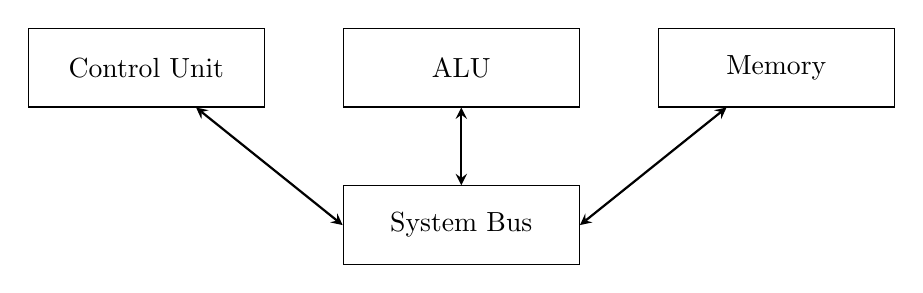
\begin{tikzpicture}[align=center,node distance=4cm]
        \node (control) [rec] {Control Unit};
        \node (alu) [rec, right of=control] {ALU};
        \node (memory) [rec, right of=alu] {Memory};
        \node (bus) [rec, below of=alu, node distance=2cm] {System Bus};
        \draw [darrow] (control) -- (bus.west);
        \draw [darrow] (alu) -- (bus);
        \draw [darrow] (memory) -- (bus.east);
    \end{tikzpicture}
    \caption{Description of the von Neumann architecture.\label{fig:vonNeumann}}
\end{figure}

Before the invention of the \gls{von Neumann architecture}, computers used discrete plugboard wiring or fixed
control circuitry to store the entire program. Examples of this persist in modern times, such as simple non-graphing calculators 
where the software cannot be updated. Reprogramming early fixed-program machines required redesign of the whole 
system. The \gls{von Neumann architecture} allowed for programs to be defined by a set of instructions (\gls{isa})
and for the program to be stored in a memory to be executed. The term \gls{stored program computer} was coined to refer 
to computers that could a program stored in its memory. 

An overview is given in Figure \ref{fig:vonNeumann}. The main components are connected by a shared bus. %
%
The term \gls{von Neumann architecture} has evolved to refer to any \gls{stored program computer} in which an 
instruction fetch and a data operation cannot occur at the same time (since they share a common bus). 
%The next instruction to be executed is located in memory. Executing the instruction requires de-referencing
%the \acrshort{ip}, placing the result in the instruction register, and the control unit setting the
%operation of the microprocessor. These operations happen in sequence. Thus, the microprocessor cannot manipulate 
%the data memory without the control unit first understanding the nature of the instruction. 
This is referred to as the von Neumann bottleneck, which often limits the performance of the corresponding 
system. %
There are other architecture designs such as the \gls{Harvard architecture} which distinguishes between 
memory for data and instructions. It called for separate busses to access instructions and data. However, 
the vast majority of microprocessors developed in the 21st century have followed the \gls{von Neumann architecture}. %
%
%To somewhat
 complicate matters, modern microprocessors include a \gls{cache} to speed up memory operations.
%Current \gls{cache} models separate instructions from data, leading to designs that distinguish between 
%memory for instructions or data. The lines between the \gls{von Neumann architecture} and 
%\gls{Harvard architecture} may be a bit blurred.

%\begin{figure}[b]
%    \myaside{Why is it called \gls{x64} if it's an Intel processor?}{%
%    \gls{x86} is a \gls{cisc} originally developed by Intel in 1978. It was iterated over many %
%    decades, with AMD as their chief competitor, offering alternative \gls{x86} compatible processors. However, in 2001, when promoting the %
%    design to 64-bit, Intel decided to push a new \gls{isa} that was not backward compatible with previous %
%    designs called \gls{ia64}. In 2003, AMD provided an alternative 64-bit version of \gls{x86} that was backward%
%    compatible. Since \gls{ia64} was not backward compatible, it required software developers to ship two executable % 
%    versions: one for legacy \gls{x86} systems and one for \gls{ia64} systems. Software developers who wanted legacy %
%    support could instead write their program in \gls{x86}, and it could run on an \gls{x64} system due to its backward % 
%    compatability. Over time, develops favored the later solution, leading to the demise of \gls{ia64} in 2020.}
%\end{figure}


\section{Arithmetic Logic Unit\label{sec:alu}}

In computing, an \gls{arithmetic logic unit} is a digital circuit that performs arithmetic and bitwise operations 
on integer binary numbers. Because binary numbers are a positional numbering system it implements positional 
arithmetic algorithm (carry-in/out) at the hardware level. %
This is in contrast to a \gls{floating point unit}, which operates on floating point 
numbers which is beyond the scope of this class. \glspl{arithmetic logic unit} are a fundamental building block of many types of computing 
circuits, including the microprocessor, \gls{floating point unit}, and \gls{gpu}. 

Some of the operations a \gls{aarch64} processor can carry out are:

\begin{itemize}
    \item Simple arithmetic operations, such as addition, subtraction, division, negation, etc. 
    \item Complex arithmetic operations consisting of multiple types of operation. For example, the \texttt{madd} 
     operation multiplies two operands, adds a third, and stores the result in a forth.
    \item Instructions to move values between registers.
    \item Evaluating the expression of a conditional branch.
\end{itemize}

The inputs to an ALU are the data to be operated on, called operands, and a \gls{opcode} indicating the operation to be 
performed; the ALU's output is the result of the performed operation. In many designs, the ALU also has status 
inputs or outputs and control lines. Status inputs or outputs convey information about a previous operation 
or the current operation, respectively, between the ALU and external status registers. Control lines are additional 
data beyond the \gls{opcode} to ensure the correct operation is carried out. With \glspl{load-and-store}, the type 
of microprocessor architecture we will study in class, the \gls{arithmetic logic unit} can only perform 
operations on values in \glspl{register}, a special type of memory.

\subsection{Registers\label{sec:alu:reg}}

\Glspl{register} are a concept perhaps unknown to individuals who have just completed their 
introductory programming courses. A processor \gls{register} is a quickly accessible location available 
to a computer's processor. %
It is faster than memory due to modern microprocessors using \gls{sram} memory technology for registers. %
There are a fixed number of registers. Each register is fixed in size. Registers used by the program are 
general purpose, although some registers 
have specific hardware functions, and may be read-only or write-only. Some common purposes for registers are given below:
%
\begin{itemize}
    \item Scratch registers are for general purpose use.
    \item Reserved registers used by the operating system that should not be modified by the program.
    \item Flag registers that cannot be modified directly but hold important information such as if overflow occured. These are often used when handling exceptions.
    \item Reference values that will always be a fixed value when used as an operand, such as zero.
    \item Pointers to important parts of memory, e.g. the next instruction, the bottom of the stack, where to return from a subroutine.
    \item Registers for passing arguments between subroutines.
\end{itemize}
%
The guidelines for using registers are defined by
a \gls{calling convention}. The registers for \gls{aarch64} are given in \ref{tab:registers}. %
%
In the past, \glspl{isa} assigned memory %
addresses to registers. With modern systems, registers have their own addressing system, ussually a 
compact addressing system with as few bits as needed. Note that the register addresses specified in 
Table \ref{tab:registers} would be given in binary.

When a program references datum in memory there is a high probability the value will be used or modified again. 
This is called \gls{temporal locality}. Random access of memory is comparatively slow in modern microprocessors 
due to the type of technology used (\gls{dram}). You will always need to reference memory at least once per datum, 
but can use registers as an intermediate structure to hold their value, reducing the number of references performed 
per program. Holding frequently used values in registers can be critical to a program's performance. Register 
allocation is performed either by a compiler in the code generation phase, or manually by an assembly language 
programmer. 

\begin{table}[t]\centering
    \caption{List of \glspl{register} in \gls{aarch64} and their purpose.\label{tab:registers}}
    \begin{tabular}{|l|l|}
        \hline Address(es) & Purpose \\\hline\hline
        31 & \Gls{sp} or \gls{reference zero} depending on context \\\hline
        30 & \Gls{ra}, used to return from subroutines \\\hline
        29 & \Gls{fp}\\\hline
        19-29 & Scratch registers, saved by the \gls{callee}\\\hline
        16-18 & Reserved\\\hline
        9-15 & Scratch registers, unsaved by the \gls{callee}\\\hline
        8 & Reserved\\\hline
        0-7 & Arguments passed for input and output with subroutines\\\hline
    \end{tabular}
\end{table}

\begin{figure}[b]
    \myaside{\gls{sram} vs. \gls{dram}}{%
    It may come as quite a shock to PC builders, but the main memory on your motherboard is too slow for the 
    microprocessor. Current memory technologies are \gls{sram}, \gls{dram} and flash. Flash is mostly used 
    for secondary storage. \gls{sram} is a type of memory technology where a single bit is constructed from 
    logic gates. It is fast, but has a comparatively high number of transistors per bit. Thus, it requires 
    a lot of physical space on the microprocessor and costs more than other technologies. \gls{dram} on the 
    other hand uses a single transistor and capacitor to represent a bit. However, due to capacitor's tendency
    to dissipate over time, \gls{dram} must be refreshed periodically. This is done in chunks, called rows. 
    The need to organize data in rows leads to a not-so-straightforeward method to randomly access data. So, 
    it is slower than \gls{sram}, but it is cheaper and requires less physical space.}
\end{figure}


\subsection{Reduced Instruction Set Computing (RISC)\label{sec:alu:risc}}

In the past, there was a need to distinguish between two different types of \glspl{isa}: %
\gls{reduced instruction set computer} and  %
\gls{complex instruction set computer}. A \gls{reduced instruction set computer} is a computer 
architecture designed %
to simplify the individual instructions given to the computer to accomplish tasks. Compared to the 
instructions given to a \gls{complex instruction set computer}, a \gls{reduced instruction set computer} might require more 
instructions (more code) in order to accomplish a task because the individual instructions are written 
in simpler code. The goal is to offset the need to process more instructions by increasing the speed 
of each instruction, in particular by implementing an instruction pipeline, which may be simpler given 
simpler instructions.

The key operational concept of the \gls{reduced instruction set computer} computer is that each instruction performs only one function 
(e.g. copy a value from memory to a register). The \gls{reduced instruction set computer} computer has tens of general-purpose 
\glspl{register} and the code uses a \gls{load-and-store} in which the code for the performing
arithmetic are separate from the instructions that grant access to memory of the computer. 
The design of the CPU allows \gls{reduced instruction set computer} computers few simple addressing modes and predictable instruction times 
that simplify design of the system as a whole.

Consider the C++ instruction \texttt{i++}. In \gls{aarch64}, a type of \gls{reduced instruction set computer}, 
this requires three instructions:
%
\begin{verbatim}
ldr w9 [x0] ; Dereference a pointer
add w9 w9 #1 ; Add one
str w9 [x0] ; Place result back into memory
\end{verbatim}
%
The first instruction fetches the value of \texttt{i} from memory. The second instruction adds one to 
the value. The third instruction stores the modified value in memory. In \gls{x64}, a type of \gls{cisc},
the same instruction is:
\begin{verbatim}
add (%rbx), 1 ; Do everything
\end{verbatim}
%
With the later example, the microprocess is instructed to increment a value in memory. It fetches the 
value, increments it, then stores the result back in memory. This is carried out using a single instruction.

It may not seem obvious why one would want a \gls{reduced instruction set computer}. However, bundling many 
atomic operations in a single hardware-level instruction increases the complexity of the design. \glspl{cisc}
tend to be more expensive, and are hard to study. With a \gls{reduced instruction set computer}, the design 
is simple enough to draw on paper. This is the why we focus on \gls{aarch64} for this introductory class.

With modern microprocessors, the lines between \gls{reduced instruction set computer} and \gls{complex instruction set computer} are
blurred. Almost all computers, whether \gls{load-and-store} or not, load data from a larger memory into registers 
where it is used for arithmetic operations and is manipulated or tested by machine instructions. Manipulated data 
is then often stored back to main memory, either by the same instruction or by a subsequent one. Finally, 
\gls{aarch64} has a few instructions that violatic the principle of single-function instructions. For example, 
a common instruction we will see in the future is:
%
\begin{verbatim}
stp x29, x30, [sp, -32]!
\end{verbatim}
%
This instruction moves the \gls{sp} by 32 bytes, and performs two register-to-memory 
storage operations, as a single hardware-level instruction. It would require more instructions to 
do this in \gls{x64} and it has no single equivalent instruction. 


\printglossary[type=\acronymtype]

\printglossary
 
\end{document}
